\subsection{Boosted Decision and Regression Trees}
\label{sec:bdt}

A {\em decision (regression) tree} is a
binary tree structured classifier (regressor) similar to the one sketched in
Fig.~\ref{fig:decisiontree}. Repeated left/right (yes/no) decisions
are taken on one single variable at a time until a stop criterion
is fulfilled.  The phase space is split this way into many regions that are
eventually classified as signal or background, depending on the
majority of training events that end up in the final {\em leaf}
node. In case of {\em regression trees}, each output node represents 
a specific value of the target variable.\footnote{The target variable 
is the variable the regression ``function'' is trying to estimate.} The
boosting (see Sec.~\ref{sec:boost}) of a decision (regression) tree extends 
this concept from one tree to several trees which form a 
{\em forest}\index{Forest}. The trees are derived from the same 
training ensemble by reweighting events, and are finally combined into a 
single classifier (regressor)
which is given by a (weighted) average of the individual decision
(regression) trees. Boosting stabilizes the response of the decision
trees with respect to fluctuations in the training sample and is able
to considerably enhance the performance w.r.t. a single tree.  In the
following, we will use the term {\em decision tree } for both, {\em
  decision-} and {\em regression trees} and we refer to regression
trees only if both types are treated differently. 
\begin{figure}[t]
  \begin{center}
          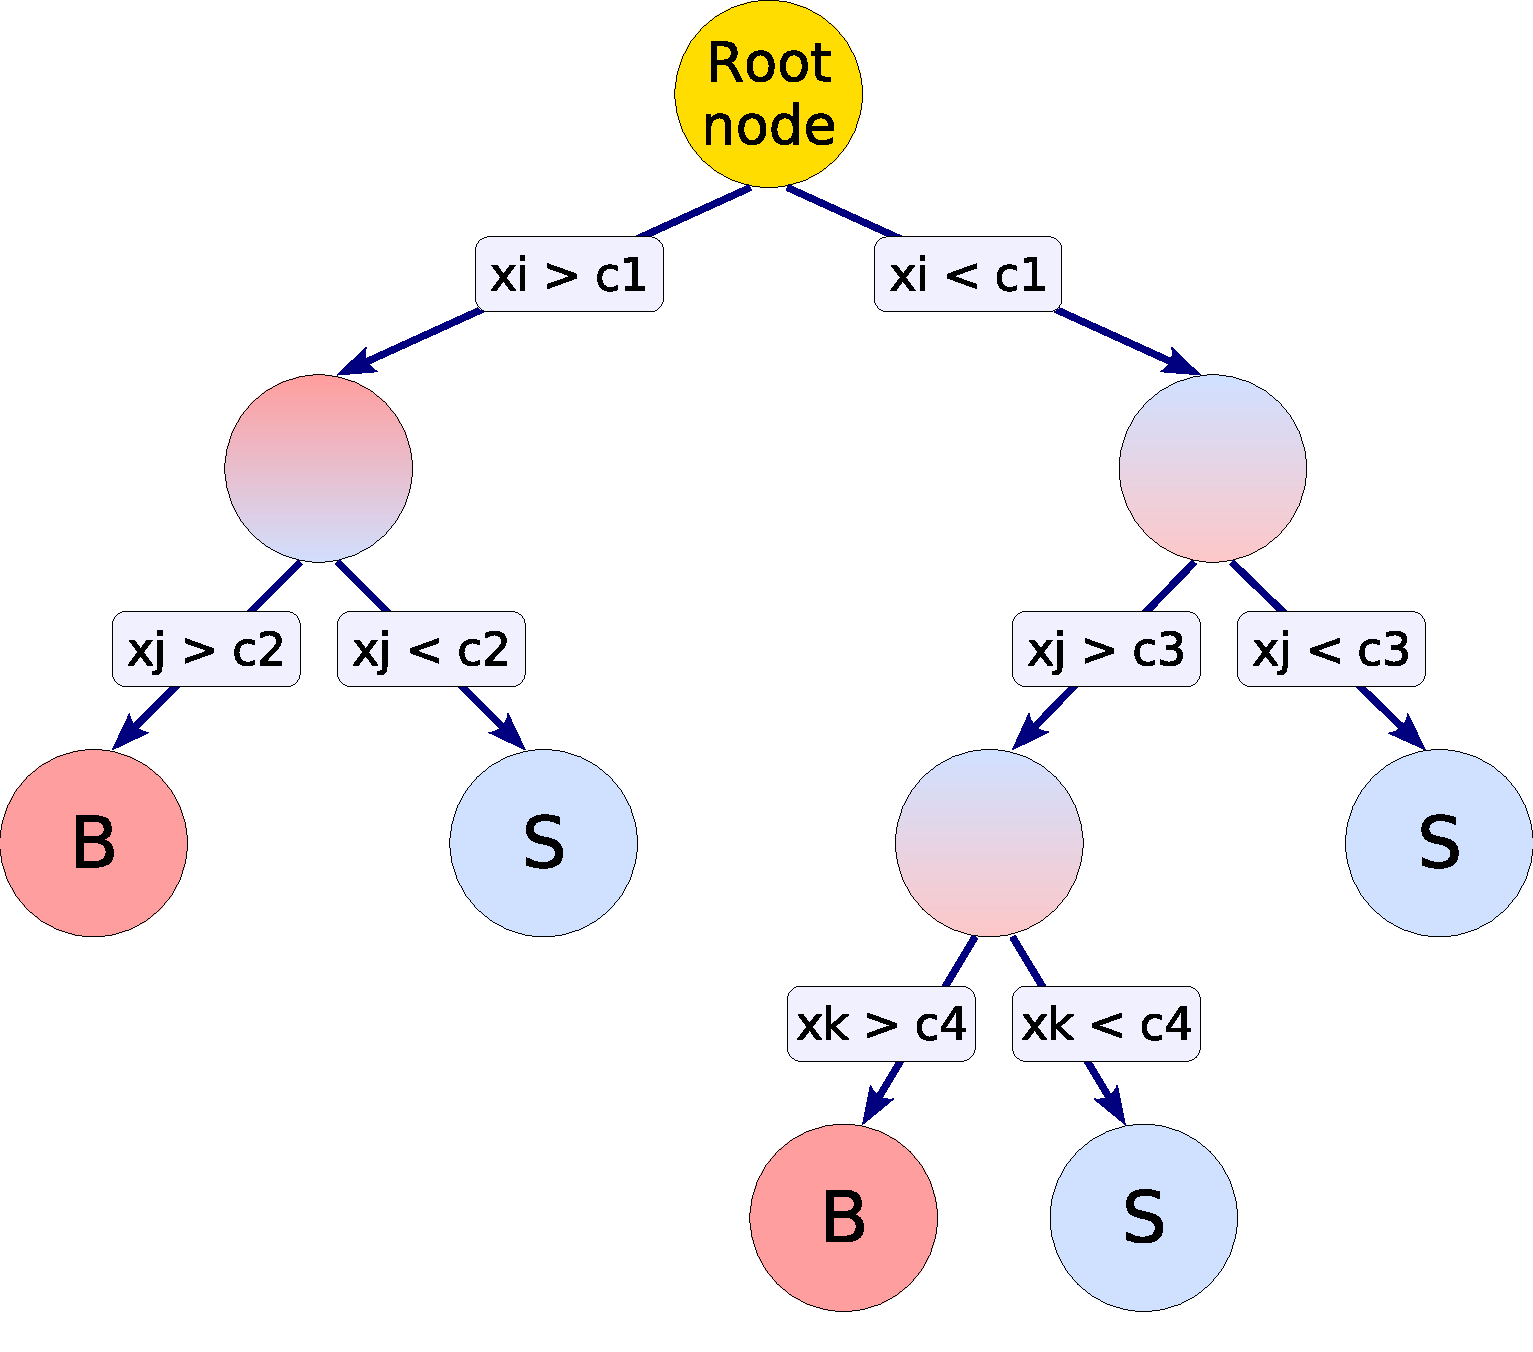
\includegraphics[width=0.60\textwidth]{plots/BDTsketch}
  \end{center}
  \vspace{-0.3cm}
  \caption[.]{Schematic view of a decision tree.  Starting from the
    root node, a sequence of binary splits using the discriminating
    variables $x_i$ is applied to the data. Each split uses the
    variable that at this node gives the best separation between
    signal and background when being cut on.  The same variable may
    thus be used at several nodes, while others might not be used at
    all.  The leaf nodes at the bottom end of the tree are labeled
    ``S'' for signal and ``B'' for background depending on the
    majority of events that end up in the respective nodes. For
    regression trees, the node splitting is performed on the variable
    that gives the maximum decrease in the average squared error when
    attributing a constant value of the target variable as
    output of the node, given by the average of the training events in
    the corresponding (leaf) node (see Sec.~\ref{sec:treebuilding}). }
\label{fig:decisiontree}
\end{figure}

\subsubsection{Booking options}

The boosted decision (regression) treee (BDT) classifier is booked via the command:
\begin{codeexample}
\begin{tmvacode}
factory->BookMethod( Types::kBDT, "BDT", "<options>" );
\end{tmvacode}
\caption[.]{\codeexampleCaptionSize Booking of the BDT classifier: 
         the first argument is a predefined enumerator, the
         second argument is a user-defined string identifier, and the third
         argument is the configuration options string. 
         Individual options are separated by a ':'. See 
         Sec.~\ref{sec:usingtmva:booking} for more information on the booking.}
\end{codeexample}
% ======= input option table ==========================================
\begin{option}[p]
\input optiontables/MVA__BDT_1.tex
\caption[.]{\optionCaptionSize Configuration options reference for MVA
  method: {\em BDT}.  Values given are defaults. If predefined
  categories exist, the default category is marked by a '$\star$'. The
  options in Option Table~\ref{opt:mva::methodbase} on
  page~\pageref{opt:mva::methodbase} can also be configured. The table
  is continued in Option Table~\ref{opt:mva::bdt_2}.  }
\label{opt:mva::bdt_1}
\end{option}

\begin{option}[p]
\input optiontables/MVA__BDT_2.tex
\caption[.]{\optionCaptionSize 
     Continuation of Option Table~\ref{opt:mva::bdt_1}.     
}
\label{opt:mva::bdt_2}
\end{option}

\begin{option}[p]
\input optiontables/MVA__BDT_3.tex
\caption[.]{\optionCaptionSize 
  Some deprecated options for the BDT
  Method that are for the moment still kept for compatibility.  }
\label{opt:mva::bdt_2}
\end{option}

Several configuration options are available to customize the BDT
classifier. They are summarized in Option Tables~\ref{opt:mva::bdt_1}
and \ref{opt:mva::bdt_2} and described in more detail in
Sec.~\ref{sec:bdt_descr}.

\subsubsection{Description and implementation}
\label{sec:bdt_descr}

Decision trees are well known classifiers that allow a straightforward
interpretation as they can be visualized by a simple two-dimensional
tree structure. They are in this respect similar to rectangular cuts.
However, whereas a cut-based analysis is able to select only {\em one}
hypercube as region of phase space, the decision tree is able to split
the phase space into a large number of hypercubes, each of which is
identified as either ``signal-like'' or ``background-like'', or
attributed a constant event (target) value in case of a regression
tree. For classification trees, the path down the tree to each leaf
node represents an individual cut sequence that selects signal or
background depending on the type of the leaf node.
 
A shortcoming of decision trees is their instability with respect to 
statistical fluctuations in the training sample from which the tree
structure is derived. For example, if two input variables exhibit
similar separation power, a fluctuation in the training sample may cause the 
tree growing algorithm to decide to split on one variable, while the other 
variable could have been selected without that fluctuation. In
such a case the whole tree structure is altered below this node,
possibly resulting also in a substantially different classifier response.

This problem is overcome by constructing a forest\index{Forest} of
decision trees and classifying an event on a majority vote of the
classifications done by each tree in the forest. All trees in the
forest are derived from the same training sample, with the events
being subsequently subjected to so-called boosting
(see~\ref{sec:boost}), a procedure which modifies their weights in the
sample. Boosting increases the statistical stability of the classifier
and is able to drastically improve the separation performance compared
to a single decision tree.  However, the advantage of the
straightforward interpretation of the decision tree is lost. While one
can of course still look at a limited number of trees trying to
interpret the training result, one will hardly be able to do so for
hundreds of trees in a forest. Nevertheless, the general structure of
the selection can already be understood by looking at a limited number
of individual trees.  In many cases, the boosting performs best if
applied to trees (classifiers) that, taken individually, have not much
classification power. These so called ``weak classifiers'' are small
trees, limited in growth to a typical tree depth of as small as two,
depending on the how much interaction there is between the different
input variables. By limiting the tree depth during the tree building 
process (training), the tendency of overtraining for simple decision
trees which are typically grown to a large depth and then pruned, is
almost completely eliminated.

\subsubsection{Boosting, Bagging and Randomising}

The different ``boosting'' algorithms (in the following we will 
call also baggand and randomised trees ``boosted'') available
for decision trees in TMVA are currently:
\begin{itemize}
\item AdaBoost (Discreate AdaBoost, see Sec.~\ref{sec:adaboost}),  RealAdaBoost (see below and \cite{RealAdaBoost}) and AdaBoostR2(see Sec.~\ref{eq:adaboostr2}) for regression
\item Gradient Boost (see Sec.~\ref{sec:gradientboost})
\item Bagging (see Sec.~\ref{sec:bagging})
\item Randomised Trees\index{Randomising}, like the Random Forests of L.~Breiman~\cite{Breiman2001}. 
  Each tree is grown in such a way that at each split only a random
  subset of all variables is considered. Moreover, each tree in the forest
  is grown using only a (resampled) subset of the original training events.
  The size of the subset as well as the number of variables considered at each
  split can be set using the options~\code{UseNTrainEvents} and \code{UseNVars}.
\end{itemize}

A possible modification of Eq.~(\ref{eq:adaboost}) for the result of
the combined classifier from the forest is to use the training
purity\footnote { The purity of a node is given by the ratio of signal
  events to all events in that node. Hence pure background nodes have
  zero purity.  }  in the leaf node as respective signal or background
{\em weights} rather than relying on the binary decision. This is then
called Real-AdaBoost can be chosen as one of the boost algorithms. For
other boosting algorithms rather than AdaBoost, the same averaging of
the individual trees can be chosen using the option
\code{UseYesNoLeaf=False} .


\subsubsection*{Training (Building) a decision tree}
\label{sec:treebuilding}

The training, building or {\em growing} of a decision tree is the
process that defines the splitting criteria for each node. The
training starts with the root node, where an initial splitting
criterion for the full training sample is determined. The split
results in two subsets of training events that each go through the
same algorithm of determining the next splitting iteration. This
procedure is repeated until the whole tree is built. At each node, the
split is determined by finding the variable and corresponding cut
value that provides the best separation between signal and background.
The node splitting stops once it has reached the minimum number
of events which is specified in the BDT configuration (option
\code{nEventsMin}).  The leaf nodes are classified as signal or
background according to the class the majority of events belongs to.
If the option \code{UseYesNoLeaf} is set the end-nodes are classified
in the same way. If \code{UseYesNoLeaf} is set to false the end-nodes
are classified according to their purity.
 
A variety of separation criteria can be configured (option
\code{SeparationType} see Option Table~\ref{opt:mva::bdt_2}) 
to assess the performance of a variable and a specific cut requirement. Because a
cut that selects predominantly background is as valuable as one that
selects signal, the criteria are symmetric with respect to the event
classes. All separation criteria have a maximum where the samples are
fully mixed, \ie, at purity $p = 0.5$, and fall off to zero when the
sample consists of one event class only.  Tests have revealed no
significant performance disparity between the following separation
criteria:
\begin{itemize}

\item {\em Gini Index} [default], defined by $p\cdot ( 1 - p )$; \index{Gini Index}

\item {\em Cross entropy}, defined by $-p \cdot \ln (p) - (1-p)\cdot \ln(1-p)$; \index{Cross Entropy}

\item {\em Misclassification error}, defined by $1-{\rm max}(p, 1-p)$; \index{Misclassification error}

\item {\em Statistical significance}, defined by $S/\sqrt{S+B}$;

\item {\em Average squared error}, defined by $1/N\cdot \sum^N (y - {\hat y})^2$ 
  for regression trees where y is the regression target of each event in the node
  and $\hat y$ is its mean value over all events in the node (which would be the
  estimate of y that is given by the node).   
\end{itemize}
Since the splitting criterion is always a cut on a single variable,
the training procedure selects {\em the} variable and cut value that
optimises the {\em increase} in the separation index between the
parent node and the sum of the indices of the two daughter nodes,
weighted by their relative fraction of events. The cut values are
optimised by scanning over the variable range with a granularity that
is set via the option \code{nCuts}. The default value of
\code{nCuts=20} proved to be a good compromise between computing time
and step size. Finer stepping values did not increase noticeably the
performance of the BDTs. However, a truly optimal cut, given the training
sample, is determined by setting \code{nCuts=-1}. This invokes an algorithm
that tests all possible cuts on the training sample and finds the best one.
The latter is of course ``slightly'' slower than the coarse grid.

In principle, the splitting could continue until each leaf node
contains only signal or only background events, which could suggest
that perfect discrimination is achievable.  However, such a decision
tree would be strongly overtrained.  To avoid overtraining a decision
tree must be {\em pruned}.

\subsubsection*{Pruning a decision tree}

Pruning\index{Pruning} is the process of cutting back a tree from the
bottom up after it has been built to its maximum size. Its purpose is
to remove statistically insignificant nodes and thus reduce the
overtraining of the tree. For simple decision trees It has been found
to be beneficial to first grow the tree to its maximum size and then
cut back, rather than interrupting the node splitting at an earlier
stage. This is because apparently insignificant splits can
nevertheless lead to good splits further down the tree. For Boosted Decision trees
however, as the boosting algorithms perform best on weak classifiers, pruning
is unnecessary as one should rather drastically limit the tree depth far 
stronger than any pruning algorithm would do afterwards. Hence, while pruning
algorithms are still implemented in TMVA, they are obsolete as they should
not be used.
%
%currently implements two tree pruning algorithms, which are set by
%option \code{PruneMethod}.
%\begin{itemize}
%
%\item Option \code{PruneMethod=ExpectedError}. For the {\em expected error pruning}~\cite{Quinlan} all leaf nodes for which
%      the statistical error estimates of the parent nodes are smaller than
%      the combined statistical error estimates of their daughter nodes are
%      recursively deleted.  The statistical error
%      estimate of each node is calculated using the binomial error
%      $\sqrt{p\cdot(1-p)/N}$, where $N$ is the number of training events
%      in the node and $p$ its purity.  The amount of pruning is controlled by
%      multiplying the error estimate by the fudge factor \code{PruneStrength}.
%      Expected error pruning is not available for the regression trees.
%
%\item Option \code{PruneMethod=CostComplexity}. {\em Cost complexity pruning}~\cite{Breiman1984} relates the
%  number of nodes in a subtree below a node to the gain in terms of
%  misclassified training events by the subtree compared to the node
%  itself with {\em no} further splitting. The cost estimate $R$ chosen
%  for the misclassification of training events is given by the
%  misclassification rate $1-{\rm max}(p, 1-p)$ in a node. The cost
%  complexity for this node is then defined by \beq \rho =
%  \frac{R(\mbox{node})-R(\mbox{subtree below that node})}
%       {\#\mbox{nodes}(\mbox{subtree below that node}) -1} \,.  \eeq
%       The node with the smallest $\rho$ value in the tree is
%       recursively pruned away as long as $\rho < {\tt
%         PruneStrength}$.
%       While for classification trees, one typically uses just the misclassification
%       error in the pruning, but Gini-Index for the node splitting, regression trees use in
%       both cases the squared error loss.
%\end{itemize}
%Note that the pruning is performed {\em after} the boosting so that
%the error fraction used by AdaBoost is derived from the unpruned tree.
% 
%If the \code{PruneStrength} option is set to a negative value, an
%algorithm attempts to automatically detect the optimal strength
%parameter. The training sample is divided into two subsamples, of
%which only one is used for training, while the other one serves for
%validation. The tree is pruned sequentially starting from the node which
%has the smallest value of the cost-complexity in the tree. After each pruning
%step the performance of the tree is assessed using the validation sample. This
%process is repeated until the ROOT node would be pruned. As optimal 
%prune strength for this tree the value is chose which corresponds to the best
%performing tree using the validation sample.
%
%While this type of pruning obviously gives the ``optimally pruned tree'' given
%the training data, it is not completely clear yet if this also applies for the
%tree in the forest. Currently it looks as if in TMVA, better results for the
%whole forest are often achieved when pruning is not applied, but rather the
%maximal tree depth is set to a relatively small value (3 or 4) already during
%the tree building phase. 
%
%Note that the Gradient boost does not apply a pruning algorithm
%and ignores option \code{PruneMethod}. In this case it is recommended
%that the user restricts the number of nodes in the tree to values
%between 5 to 20 by using option \code{NNodesMax} or the maximal allowed depth of the
%tree \code{MaxDepth}.

\subsubsection{Variable ranking}

A ranking of the BDT input variables is derived by counting how often the
variables are used to split decision tree nodes, and by weighting each 
split occurrence by the separation gain-squared it has achieved and by 
the number of events in the node~\cite{Breiman1984}. This measure of the
variable importance can be used for a single decision tree as well as for a 
forest.

\subsubsection{Performance}

Only limited experience has been gained so far with boosted decision
trees in HEP. In the literature decision trees are sometimes referred
to as the best ``out of the box'' classifiers. This is because little
tuning is required in order to obtain reasonably good results. This is
due to the simplicity of the method where each training step (node
splitting) involves only a one-dimensional cut optimisation. Decision
trees are also insensitive to the inclusion of poorly discriminating
input variables. While for artificial neural networks it is typically
more difficult to deal with such additional variables, the decision
tree training algorithm will basically ignore non-discriminating
variables as for each node splitting only the best discriminating
variable is used.  However, the simplicity of decision trees has the
drawback that their theoretically best performance on a
given problem is generally inferior to other techniques like neural
networks. This is seen for example using the academic training samples
included in the TMVA package. For this sample, which has equal RMS but
shifted mean values for signal and background and linear correlations
between the variables only, the Fisher discriminant provides
theoretically optimal discrimination results. While the artificial
neural networks are able to reproduce this optimal selection
performance the BDTs always fall short in doing so. However, in other
academic examples with more complex correlations or real life
examples, the BDTs often outperform the other techniques.  This is
because either there are not enough training events available that
would be needed by the other classifiers, or the optimal configuration
(\ie\ how many hidden layers, which variables) of the neural network
has not been specified. We have only very limited experience at the
time with the regression, hence cannot really comment on the performance
in this case.

